\documentclass{article}

\usepackage[italian]{babel}
\usepackage[margin=2cm, footskip=5mm]{geometry}
% questi package non sono necessari in lualatex; ref https://tex.stackexchange.com/a/413046
% \usepackage[utf8]{inputenc}
% \usepackage[T1]{fontenc}
\usepackage{enumitem}
\usepackage{hyperref}
\usepackage{titlesec}
\usepackage{soulutf8}
\usepackage{contour}
\usepackage{float}
\usepackage{graphicx}
\usepackage{fancyhdr}
\usepackage{longtable}
\usepackage[table]{xcolor}
\usepackage{titling}
\usepackage{lastpage}
\usepackage{ifthen}
\usepackage{calc}
\usepackage{minted}
\usepackage{pgfgantt}
\usepackage{subfiles}

\newlength{\imgwidth}

\newcommand\scalegraphics[1]{%
    \settowidth{\imgwidth}{\includegraphics{#1}}%
    \setlength{\imgwidth}{\minof{\imgwidth}{\textwidth}}%
    \includegraphics[width=\imgwidth]{#1}%
}

% XXX definizione dei percorsi in cui cercare immagini
\graphicspath{ {./}
    {./img/}
}

% esempio di utilizzo: \appendToGraphicspath{./img/} (un comando diverso per ogni path da includere)
% N.B.: ci DEVE essere un forward slash alla fine del path, a indicare che è una cartella.
\makeatletter
\newcommand\appendToGraphicspath[1]{%
  \g@addto@macro\Ginput@path{{#1}}%
}
\makeatother

% setup della sottolineatura
\setuldepth{Flat}
\contourlength{0.8pt}

\newcommand{\uline}[1]{%
  \ul{{\phantom{#1}}}%
  \llap{\contour{white}{#1}}%
}

% setup dei link
\hypersetup{
  colorlinks=true, % set true if you want colored links
  linktoc=all,     % set to all if you want both sections and subsections linked
  linkcolor=black, % choose some color if you want links to stand out
}

% setup di header e footer
\pagestyle{fancy}

\fancyhf{}
\fancyhead[L]{\includegraphics[width=1cm]{logo.png}}
\fancyhead[R]{\thetitle}
\fancyfoot[R]{\thepage\ di~\pageref{LastPage}}

\fancypagestyle{nopage}{%
  \fancyfoot{}%
}

\setlength{\headheight}{1.2cm}

% setup forma \paragraph e \subparagraph
\titleformat{\paragraph}[hang]{\normalfont\normalsize\bfseries}{\theparagraph}{1em}{}
\titleformat{\subparagraph}[hang]{\normalfont\normalsize\bfseries}{\thesubparagraph}{1em}{}

% setup profondità indice di default
\setcounter{secnumdepth}{5}
\setcounter{tocdepth}{5}

% shortcut per i placeholder
\newcommand{\plchold}[1]{\textit{\{#1\}}} % chktex 20

% hook per lo script che genera il glossario
\newcommand{\glossario}[1]{\underline{#1}\textsubscript{g}}

% definizione dei comandi \uso e \stato
\makeatletter
\newcommand{\setUso}[1]{%
  \newcommand{\@uso}{#1}%
}
\newcommand{\uso}{\@uso}

\newcommand{\setStato}[1]{%
  \newcommand{\@stato}{#1}%
}
\newcommand{\stato}{\@stato}

\newcommand{\setVersione}[1]{%
  \newcommand{\@versione}{#1}%
}
\newcommand{\versione}{\@versione}

\newcommand{\setResponsabile}[1]{%
  \newcommand{\@responsabile}{#1}%
}
\newcommand{\responsabile}{\@responsabile}

\newcommand{\setRedattori}[1]{%
  \newcommand{\@redattori}{#1}%
}
\newcommand{\redattori}{\@redattori}

\newcommand{\setVerificatori}[1]{%
  \newcommand{\@verificatori}{#1}%
}
\newcommand{\verificatori}{\@verificatori}

\newcommand{\setDescrizione}[1]{%
  \newcommand{\@descrizione}{#1}%
}
\newcommand{\descrizione}{\@descrizione}

\newcommand{\setModifiche}[1]{%
  \newcommand{\@modifiche}{#1}%
}

\newcommand{\modifiche}{\@modifiche}

\makeatother

% setup delle description
\setlist[description,1]{font=$\bullet$\hspace{1.5mm}, labelwidth=* leftmargin=*,labelindent=12.5mm}
\setlist[description,2]{font=$\bullet$\hspace{1.5mm}, leftmargin=*,labelindent=12.5mm}
\appendToGraphicspath{../../commons/img/}

\title{Verbale esterno --- 25/02/2020}

\setResponsabile{Alessandro Rizzo}
\setRedattori{Alessandro Rizzo}
\setVerificatori{ Alberto Cocco }
\setUso{Esterno}
\setDescrizione{Verbale dell'incontro di GruppOne del 25/02/2020}
\setModifiche{%
\cellcolor{white!80!lightgray!100}& Alessandro Rizzo & 2020--02--27 & approva documento \\%
\cellcolor{white!80!lightgray!100}& Alberto Cocco & 2020--02--26 & verifica verbale \\%
\multirow{-3}{*}{0.1.0}& Alessandro Rizzo & 2020--02--25 & stendi verbale %
}

\begin{document}

\thispagestyle{empty}
\pagenumbering{gobble}

\begin{center}

  \includegraphics[width=8.5cm]{\commons/img/logo.png}\\
  {\Large GruppOne - progetto "Stalker"}\\
  \vspace{1.5cm}

  {\Huge \thetitle}
  \vspace{1.5cm}

  \begin{table}[H]
    \centering

    \begin{tabular}{r|l}
      \textbf{Versione}     & \versione              \\
      \textbf{Approvazione} & \responsabile          \\
      \textbf{Redazione}    & \redattori             \\
      \textbf{Verifica}     & \verificatori          \\
      \textbf{Stato}        & \stato                 \\
      \textbf{Uso}          & \uso                   \\
      \textbf{Destinato a}  & Imola Informatica      \\
                            & GruppOne               \\
                            & Prof. Tullio Vardanega \\
                            & Prof. Riccardo Cardin  \\
    \end{tabular}
  \end{table}

  \vspace{3cm}
  \textbf{Descrizione}\\
  \descrizione\\
  \vfill
  \verb|gruppone.swe@gmail.com|
\end{center}

\newpage
\thispagestyle{nopage}

\section*{Registro delle modifiche}
\label{sec:registro_delle_modifiche}

\begin{table}[H]
  \label{tab:registro_delle_modifiche}

  \centering
  \rowcolors{2}{lightgray}{white!80!lightgray!100}

  \begin{longtable}[c]{c c c c l}
    \rowcolor{darkgray!90!}\color{white}{\textbf{Versione}} & \color{white}{\textbf{Data}} & \color{white}{\textbf{Nominativo}} & \color{white}{\textbf{Ruolo}} & \color{white}{\textbf{Descrizione}} \\\endhead
    \modifiche
  \end{longtable}
\end{table}

% section registro_delle_modifiche (end)
\newpage

\thispagestyle{nopage}
\pagenumbering{roman}
\tableofcontents

\newpage

\pagenumbering{arabic}


\section{Informazioni logistiche}%
\label{sec:informazioni_logistiche}

\begin{description}
  \item [Luogo] chiamata Hangouts
  \item [Data] 25/02/2020
  \item [Ora] 12:30 \symbol{8594} 12:55
\end{description}

\subsection{Membri del gruppo presenti}%
\label{sub:membri_del_gruppo_presenti}

\begin{enumerate}
  \item Alberto Cocco
  \item Luca Ercole
  \item Alberto Gobbo
  \item Alessandro Rizzo
\end{enumerate}
% sub:membri_del_gruppo_presenti (end)

\subsection{Altri partecipanti}%
\label{sub:altri_partecipanti}

\begin{enumerate}
  \item Prof.\ Riccardo Cardin (committente)
\end{enumerate}

% sub:altri_partecipanti (end)
% sec:informazioni_logistiche (end)

\section{Introduzione}%
\label{sec:introduzione}

L'incontro, avvenuto tramite chiamata Hangouts, ci è servito per chiarire i dubbi riguardanti il giudizio ricevuto in RR e approfondire alcuni dettagli relativi al PoC.

\section{Ordine del giorno}%
\label{sec:ordine_del_giorno}

\begin{itemize}
  \item Discussione UUC4.3
  \item Discussione AUC3
  \item Discussione sul tracciamento di casi d'uso e requisiti
  \item Struttura del PoC
  \item Tecnologie da usare nel PoC.
\end{itemize}
% sec:registro_delle_decisioni (end)
\section{Discussione UUC4.3}%
\label{sec:discussione_uuc_4.3}
\textbf{Domanda:} Il motivo per il quale vediamo UUC4.3 come un'estensione di UUC4.2, è il fatto che l'utente può selezionare una o più organizzazioni e, nel momento in cui una di queste sia privata e quindi richieda l'autenticazione LDAP, allora si scateni il caso d'uso UUC4.3.
Quindi se UUC4.3 non fosse un'estensione di UUC4.2 ma una sua pre-condizione, l'autenticazione LDAP verrebbe effettuata a priori su tutte le organizzazioni selezionate, il che sarebbe vero solo se tutte le organizzazioni lo richiedano (sia private che pubbliche), cosa che non è richiesta da capitolato (solo private), in che modo è sbagliata questa visione del caso d'uso? \\
\textbf{Risposta:} Bisogna innanzitutto capire come UML può essere utilizzato per modellare i casi d'uso, questi ultimi infatti definiscono solamente le funzionalità del nostro software. Il professore ha ribadito questo fatto per dire che la selezione di una organizzazione è un dettaglio implementativo non una funzionalità, la funzionalità offerta invece è il collegamento ad una organizzazione dunque l'estensione non ha motivo di esserci così come il caso d'uso relativo alla selezione.
In caso il modo corretto di modellare un caso d'uso di questo tipo sarebbe prevedere 4.3 come precondizione di 4.2.
% sec:discussione_uuc_4.3 (end)
\section{Discussione AUC3}%
\label{sec:discussione_auc3}
\textbf{Domanda:} \textit{AUC3: le inclusioni non sono corrette (\ldots) AUC4: inclusioni non corrette.} Non ci è chiaro il motivo per il quale le inclusioni nei seguenti casi d'uso non sono corrette.\\
\textbf{Risposta:} Analogamente a quanto scritto prima la funzionalità di selezione di organizzazione non esiste di fatto e in questo caso nemmeno l'invio di richiesta di aggiornamento delle organizzazioni è una funzionalità esprimibile nei casi d'uso poiché è una azione automatica del sistema.
Il professore ha compreso l'intento del gruppo di fornire la possibilità di collegarsi, eliminare e modificare più organizzazioni insieme e ha suggerito se si desidera implementare queste funzionalità di definirle in casi d'uso appositi (e.g. Eliminazione di più organizzazioni).
% sec:discussione_auc3 (end)

\section{Discussione tracciamento casi d'uso e requisiti}%
\label{sec:discussione_tracciamento_casi_requisiti}
\textbf{Domanda:} \textit{Manca il tracciamento tra casi d’uso e requisiti}. Anche qui non ci è chiaro esattamente che modifiche dovremmo attuare.\\
\textbf{Risposta:} Nel documento \textit{Analisi dei Requisiti v0.0.8} è presente solamente la tabella che correla i requisiti ai casi d'uso e non viceversa.
La prima correlazione ci permette di appurare che tutti i requisiti siano necessari poiché derivano da un caso d'uso, la seconda che tutti i casi d'uso siano necessari poiché si concretizzano in un requisito.
Inoltre la tabella che collega le fonti con i casi d'uso è poco indicativa e non fornisce informazioni utili.
% sec:discussione_tracciamento_casi_requisiti (end)

\section{Domanda sul PoC}%
\label{sec:domanda_poc}
\textbf{Domanda:} Qual è il nostro obiettivo con il PoC?\@ Che grado di comprensione delle tecnologie dobbiamo dimostrare di aver raggiunto?\\
\textbf{Risposta:} Il professore ci ha consigliato di raggiungere il massimo grado di integrazione tra il maggior numero di tecnologie possibili nel PoC con lo scopo di dimostrare la piena padronanza delle suddette.
% sec:domanda_poc (end)

\section{Tecnologie da utilizzare nel PoC}%
\label{sec:tecnologie_poc}
\textbf{Domanda:} Lei consiglia di utilizzare Quarkus come tecnologie contrapposto a Spring?\\
\textbf{Risposta:} Il professore non ha sconsigliato di utilizzare Quarkus ma ci ha anche fatto notare che Spring offre una integrazione con quasi ogni tecnologia.
% sec:tecnologie_poc (end)
\newpage
\section{Registro delle decisioni}%
\label{sec:registro_delle_decisioni}

\begin{table}[H]
  \centering
  \rowcolors{2}{lightgray}{white!80!lightgray!100}
  \renewcommand{\arraystretch}{2}
  \begin{tabular}{c b{13cm}}
    \rowcolor{darkgray!90!}\color{white}{\textbf{Codice}} & \color{white}{\textbf{Decisione}}\\
    1 & Correggere i casi d'uso AUC3, UUC4.3 e UUC4.2 in concordanza con quanto discusso con il Professore durante la chiamata.\\
    2 & Rivalutare la struttura e le componenti principali del PoC in base a quanto ci ha detto il Professore. \\
    3 & Scrivere la tabella che correla casi d'uso e requisiti al posto di quella con fonte e casi d'uso.\\
  \end{tabular}
  \caption{registro delle decisioni}%
  \label{tab:registro delle decisioni}
\end{table}
% sec:registro_delle_decisioni (end)

\end{document}
